% =====================================================================
%  Entregable T2(a): Evolucion temporal por integracion directa (RK4)
%  Fragmento \input-able en el documento maestro (context/doc/mpemba_cuantico.tex).
%  Las figuras se referencian relativas a context/doc/.
% =====================================================================
\section{Evolución temporal (a): integración directa con RK4}
\label{sec:t2a}

\subsection{Explicación del framework}
La tarea de \emph{evolución temporal} consiste en obtener la trayectoria del
operador densidad $\rho(t)$ que resuelve la ecuación maestra de Lindblad
$\dot\rho=\mathcal{L}[\rho]$ (ec.~\eqref{eq:gksl}) a partir de una preparación
$\rho_0$, para trazar las curvas de distancia al equilibrio
$\Dop(\rho_t\|\rss)$ que revelan (o descartan) el efecto Mpemba. El método~(a)
es la vía \textbf{directa}: integrar la ecuación diferencial paso a paso, sin
construir el superoperador $\mathbb{L}$ de dimensión $d^2\times d^2$, aplicando
en su lugar la acción \emph{matrix-free}
$\mathcal{L}[\rho]=-i[H,\rho]+\sum_\mu(L_\mu\rho L_\mu^\dagger-\tfrac12\{L_\mu^\dagger L_\mu,\rho\})$.

\subsection{Discretización y método numérico}
Se emplea el método de \textbf{Runge--Kutta clásico de 4.º orden} (RK4), un
integrador explícito de un paso. Para $\dot\rho=\mathcal{L}[\rho]$ y paso
$\Delta t$:
\begin{align*}
k_1&=\mathcal{L}[\rho_n], &
k_2&=\mathcal{L}[\rho_n+\tfrac{\Delta t}{2}k_1], &
k_3&=\mathcal{L}[\rho_n+\tfrac{\Delta t}{2}k_2], \\
k_4&=\mathcal{L}[\rho_n+\Delta t\,k_3], &
\rho_{n+1}&=\rho_n+\tfrac{\Delta t}{6}(k_1+2k_2+2k_3+k_4). &&
\end{align*}
El error local es $\mathcal{O}(\Delta t^5)$ y el global $\mathcal{O}(\Delta t^4)$.
Cada paso requiere \emph{cuatro} evaluaciones del Liouvilliano; cada evaluación,
para la cadena de Ising disipativa, son $2+3N_J$ productos de matrices densas
$d\times d$ (con $N_J=2N$ operadores de salto), de coste $\mathcal{O}(d^3)$ cada
uno. El coste por paso es por tanto $\mathcal{O}(N\,d^3)$.

\subsection{Implementación serial}
El núcleo está en \texttt{common/lindblad.hpp} (acción \texttt{apply\_lindblad},
modelo \texttt{build\_ising}, estado de Gibbs por tiempo imaginario) y el
integrador en \texttt{a\_integracion\_directa/src/rk4\_evolution.cpp}. La
preparación inicial es un estado de Gibbs a $T_0=5$ y la referencia de relajación
el estado de Gibbs del baño a $T=0{,}8$. El \emph{hotspot} absoluto es el
producto de matrices densas \texttt{matmul}.

\subsection{Justificación de la paralelización: OpenMP}
El patrón de cómputo de la integración directa es: \emph{miles de pasos
secuenciales} (dependencia temporal estricta: $\rho_{n+1}$ necesita $\rho_n$),
cada uno dominado por productos de matrices densas que reutilizan los mismos
datos. La dependencia temporal \textbf{impide} paralelizar entre pasos; el
paralelismo disponible está \emph{dentro} de cada paso, en el \texttt{matmul}.
Ese es un patrón de \textbf{memoria compartida} con datos regulares y de tamaño
moderado ($d\times d$ cabe en caché/RAM de un nodo): el paradigma natural es
\textbf{OpenMP}, paralelizando el bucle de filas del \texttt{matmul}
(\texttt{\#pragma omp parallel for}). MPI sería contraproducente aquí
(distribuir matrices pequeñas introduce comunicación de halo en cada uno de los
miles de pasos); CUDA daría más ancho de banda pero no hay GPU disponible en la
máquina de prueba (se discute como trabajo futuro en \S\ref{sec:t2b} y en la
tabla~\ref{tab:paradigma}). La corrección de la versión paralela se verifica de
forma exacta: serial y multinúcleo producen el \emph{mismo} estado final
(coincidencia a precisión de máquina del observable $D_{HS}$ final).

\subsection{Comparación serial vs paralelo}
\begin{figure}[h]
\centering
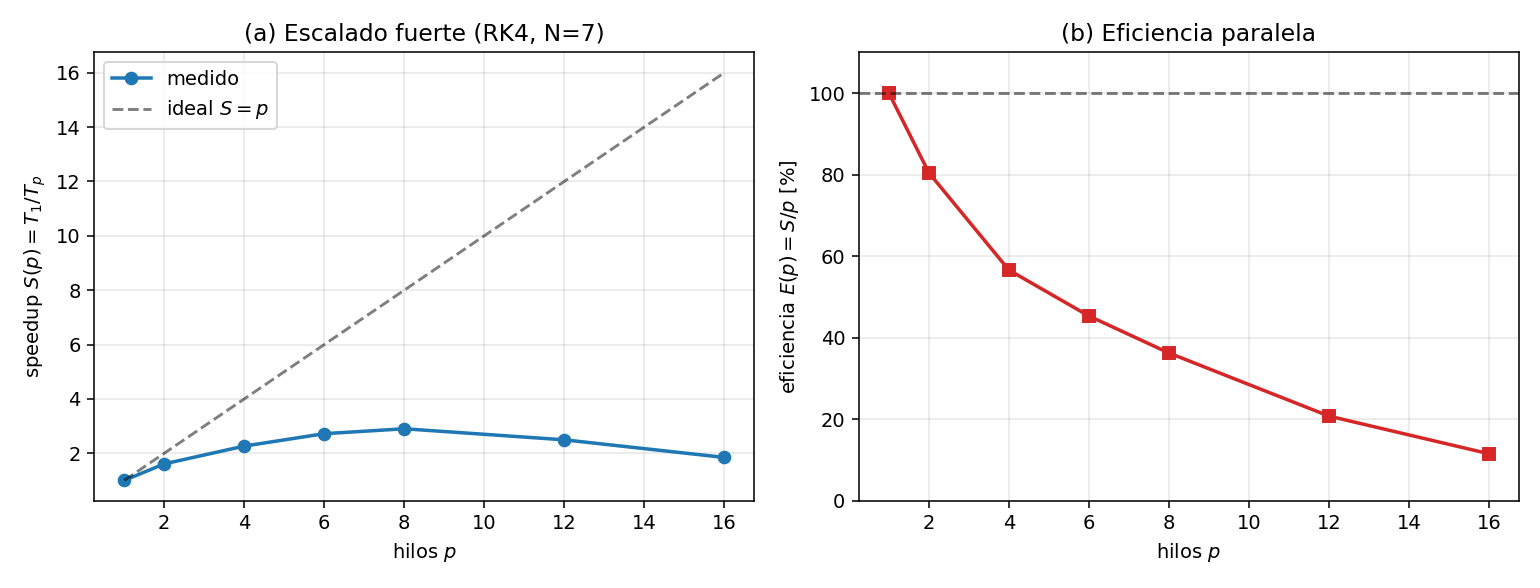
\includegraphics[width=0.92\textwidth]{../../T2/a_integracion_directa/results/fig_t2a_speedup.png}
\caption{Escalado fuerte del integrador RK4 (cadena de Ising disipativa $N=7$,
$d=128$) en un AMD Ryzen 7 7730U (8 núcleos físicos / 16 hilos). (a) speedup
$S(p)=T_1/T_p$ frente al ideal $S=p$; (b) eficiencia paralela $E(p)=S/p$.}
\label{fig:t2a_speedup}
\end{figure}

El speedup es \textbf{sublineal} y satura cerca del número de núcleos físicos: se
alcanza $S_{\max}\approx2{,}9$ con $8$ hilos, con eficiencia del
$36\,\%$ a 8 hilos. El ajuste a la \textbf{ley de Amdahl}
$S(p)=1/[f+(1-f)/p]$ da una fracción serie efectiva $f\approx0{,}25$. Las
causas de la sublinealidad son típicas de este patrón: (i)~el integrador hace
\emph{fork/join} de OpenMP en cada uno de los muchos \texttt{matmul} pequeños,
con sobrecoste acumulado; (ii)~el problema es \emph{memory-bandwidth bound}
(las matrices se releen de memoria), de modo que los hilos compiten por el
ancho de banda compartido; (iii)~las asignaciones de memoria temporales y las
operaciones vectoriales fuera del \texttt{matmul} son seriales. El salto de 8 a
16 hilos aporta poco porque los 16 hilos son \emph{hyperthreads} sobre 8 núcleos
físicos, sin ancho de banda adicional.

Para ver \emph{directamente} la mejora —y no solo el speedup adimensional— la
Figura~\ref{fig:t2a_serial_parallel} enfrenta el \textbf{tiempo de cómputo en
serie (1~hilo) y en paralelo (8~hilos)} en función del tamaño del sistema~$N$
(la malla del operador, $d=2^N$), a igual número de pasos. Ambas curvas crecen
como $\sim d^3$, pero la paralela queda sistemáticamente por debajo: la
\emph{separación} entre las dos es la ganancia, y crece con la malla porque a
mayor $d$ el \texttt{matmul} domina y amortiza mejor el coste de \emph{fork/join}.

\begin{figure}[h]
\centering
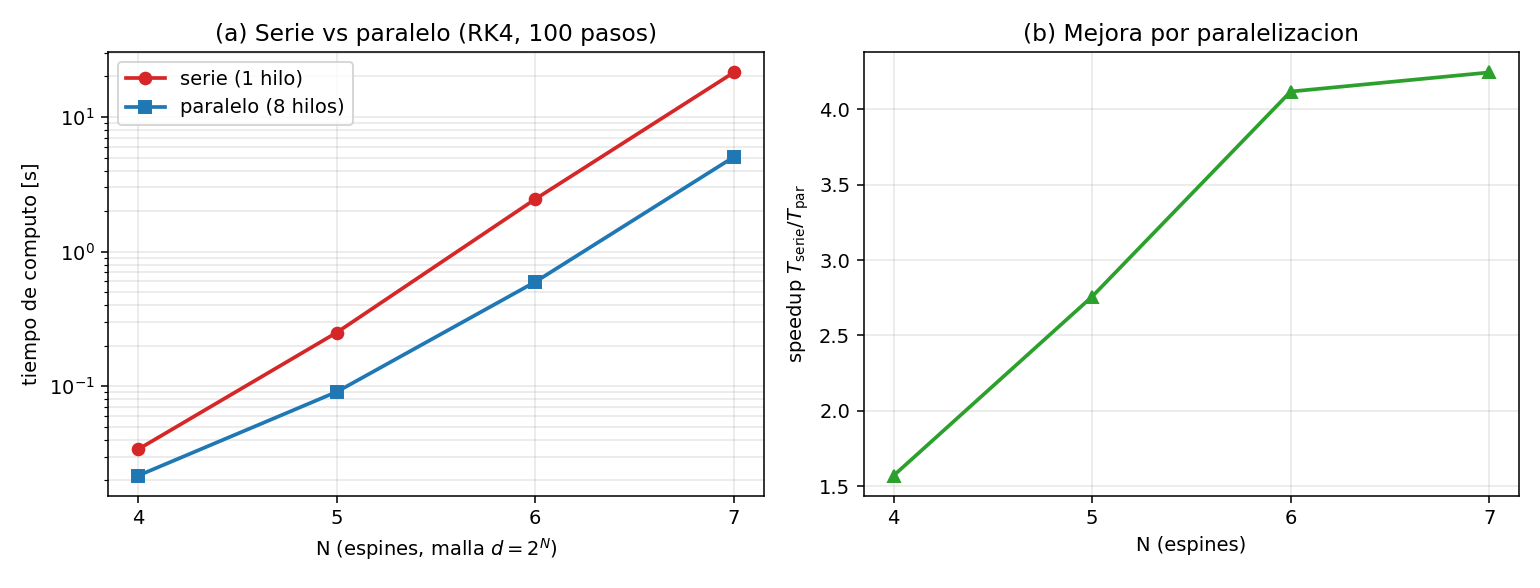
\includegraphics[width=0.92\textwidth]{../../T2/a_integracion_directa/results/fig_t2a_serial_parallel.png}
\caption{Tiempo de cómputo \textbf{serie vs paralelo} del RK4 frente al tamaño
del sistema $N$ (malla $d=2^N$), a $100$ pasos fijos. (a)~las dos curvas
($1$~hilo en rojo, $8$~hilos en azul, escala log) muestran el mismo coste
$\sim d^3$ desplazado: el hueco entre ellas es la mejora. (b)~el speedup
$T_{\mathrm{serie}}/T_{\mathrm{par}}$ resultante crece con la malla (de
$\sim\!1{,}6$ en $N=4$ a $\sim\!4$ en $N=7$): cuanto mayor es $d$, más domina el
\texttt{matmul} y mejor se amortiza el \emph{fork/join}, aunque siempre sublineal
frente al ideal de $8$.}
\label{fig:t2a_serial_parallel}
\end{figure}

\subsection{Resultados y validación}
\paragraph{Correctitud y orden del método.}
La figura~\ref{fig:t2a_convergence} valida el integrador frente a la evolución
espectral \emph{exacta} $e^{t\mathcal{L}}\rho_0$ (suma de modos): el error a
tiempo fijo decae como $\Delta t^4$, confirmando el \textbf{orden 4} del RK4
(pendiente medida $\approx4{,}04$).

\begin{figure}[h]
\centering
\begin{minipage}{0.49\textwidth}\centering
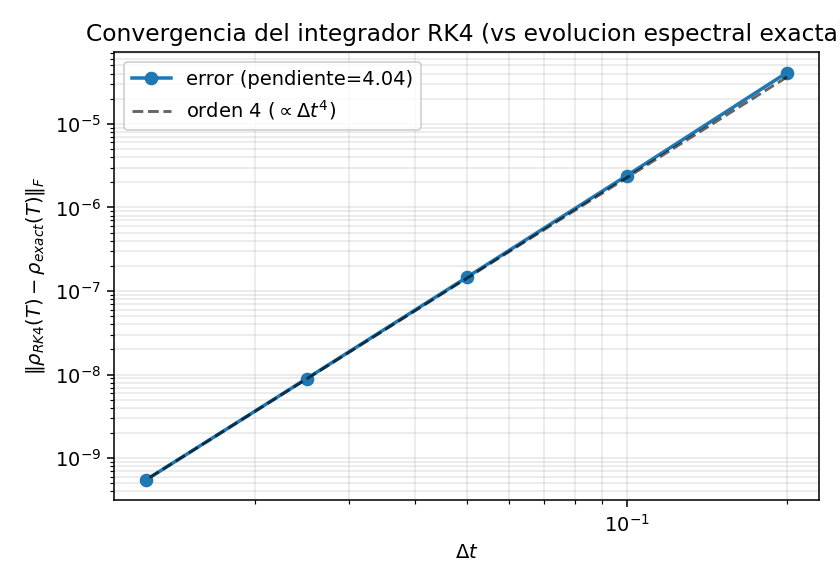
\includegraphics[width=\textwidth]{../../T2/a_integracion_directa/results/fig_t2a_convergence.png}
\end{minipage}\hfill
\begin{minipage}{0.49\textwidth}\centering
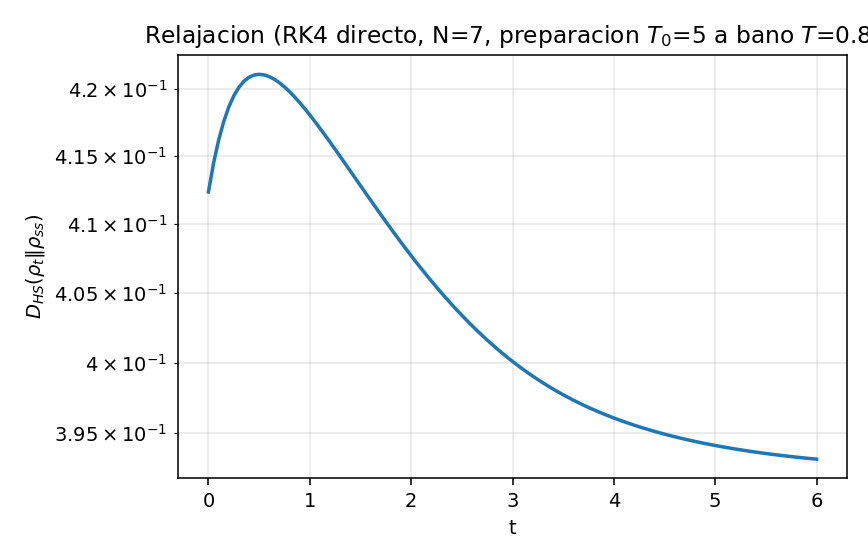
\includegraphics[width=\textwidth]{../../T2/a_integracion_directa/results/fig_t2a_relax.png}
\end{minipage}
\caption{Izquierda: convergencia de orden 4 del RK4 frente a la solución exacta.
Derecha: curva de relajación $D_{HS}(t)$ producida por el método (preparación
caliente $T_0=5$ relajando al baño $T=0{,}8$).}
\label{fig:t2a_convergence}
\end{figure}

\paragraph{Coste con el tamaño.}
La figura~\ref{fig:t2a_size} confirma el escalado $\mathcal{O}(d^3)$ por paso esperado
del producto de matrices densas: al pasar de $N$ a $N+1$ ($d\to2d$) el coste por
paso se multiplica por $\sim 8$. Es justamente este crecimiento el que vuelve
inviable la representación densa de $\rho$ para $N$ grande y motiva las
trayectorias (\S\ref{sec:t3}) en el régimen de muchos cuerpos.

\begin{figure}[h]
\centering
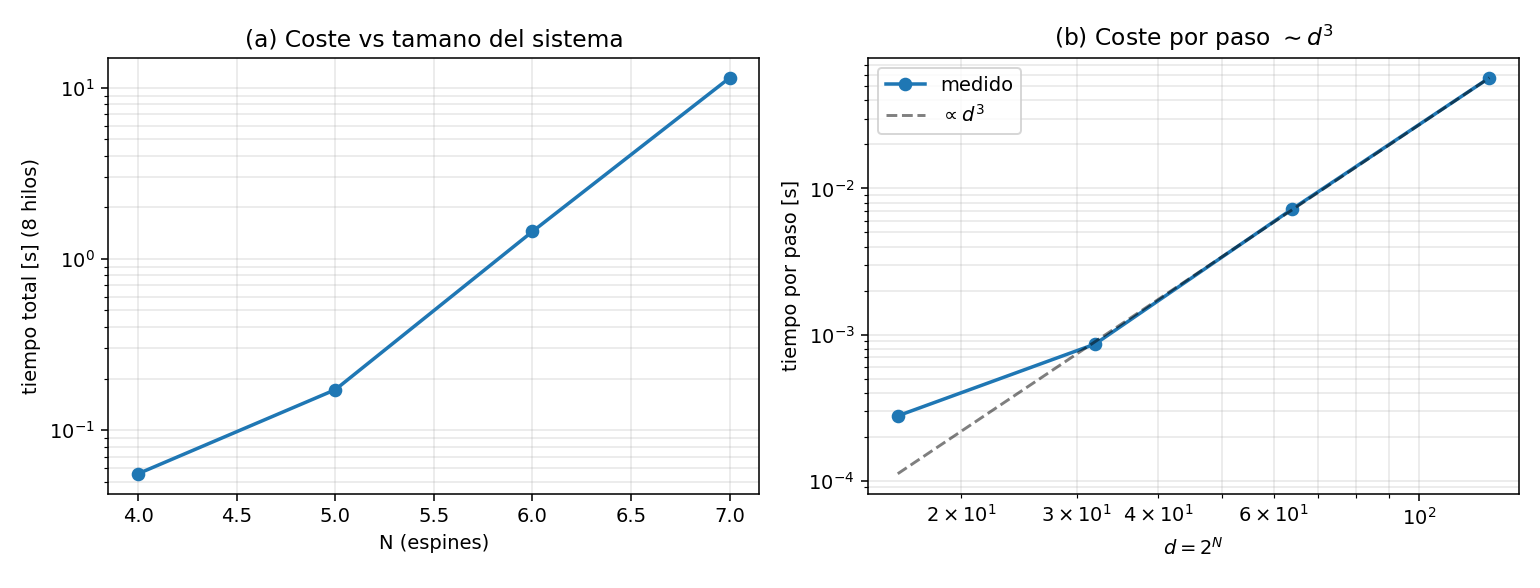
\includegraphics[width=0.92\textwidth]{../../T2/a_integracion_directa/results/fig_t2a_size.png}
\caption{Coste del método con el tamaño del sistema (8 hilos). (a) tiempo total;
(b) tiempo por paso frente a la referencia $\propto d^3$.}
\label{fig:t2a_size}
\end{figure}

\paragraph{Conclusión del método (a).}
La integración directa por RK4 es \emph{simple, exacta a orden 4 y robusta}, y se
paraleliza de forma natural con OpenMP a nivel del producto de matrices. Su
limitación es doble: el coste $\mathcal{O}(d^3)$ por paso y la necesidad de pasos
pequeños por estabilidad/precisión, que obligan a muchas evaluaciones del
Liouvilliano. El método~(b) (acción del exponencial, \S\ref{sec:t2b}) ataca
precisamente este segundo punto.
